\section{Measurement Design}
\label{sec:design}

This section defines the object we measure, the channel over which it is
measured, and the two bounds that constitute the bracket. One rule governs the
design: each side of the bracket is asserted only at the strength it can carry,
and neither side borrows strength from the other.

\subsection{Problem formulation}
\label{sec:design/problem}

Let $P$ and $Q$ be the distributions of an observable random variable for two
services $a$ and $b$. Our object is the total variation distance
\begin{equation}
  \tv(P,Q) \;=\; \tfrac{1}{2}\sum_{x} \abs{P(x) - Q(x)},
  \label{eq:tv}
\end{equation}
which lower-bounds the error of any test that distinguishes $a$ from $b$: for any
measurable test $\phi$,
$\Pr[\phi \text{ errs}] \ge \tfrac{1}{2}\bigl(1 - \tv(P,Q)\bigr)$.
A bound on $\tv$ is therefore a bound on the best achievable error, and every
statement we make about distinguishability is phrased in those terms.

We report a two-sided interval
\begin{equation}
  \epslo \;\le\; \tv(P,Q) \;\le\; \epshi ,
  \label{eq:bracket}
\end{equation}
where the two endpoints come from different statistical machinery and carry
different guarantees. $\epshi$ is a finite-sample upper bound at a stated
confidence level; $\epslo$ is an asymptotic lower bound. The interval is
certified for a pair when both endpoints exist and satisfy the gate
\begin{equation}
  \epslo > 0.05 \quad\text{and}\quad \epshi < 0.5 .
  \label{eq:gate}
\end{equation}
The gate is a conjunction, and we name both of its conditions wherever we report
a count, because a bound that clears one condition and not the other is not a
certificate. \Cref{fig:bracket} shows the pipeline end to end.

\subsection{Channel definition and hygiene}
\label{sec:design/channel}

The observable is a prefix of the packet sequence, represented by the pair
(direction, size) of each packet. We quantize each axis into $M$ bins and take
the first $k$ positions, giving an alphabet of $m = (2M)^k$ symbols. The rung
ladder is $M \in \{1,2,4,8,16\}$ and $k \in \{5,10,15,30\}$. We treat $M$ as a
discrete rung rather than a continuous knob, because the interesting behavior is
at the coarse end and a continuous sweep would obscure it.

Two properties of this channel matter for interpretation. It is coarse by
construction. The exporter we use also exposes inter-packet timing, and we
exclude it; no name, address, user-agent, or TLS-extension field is consumed by
any measurement in this paper. Second, the alphabet size $m$ is the a-priori grid
size and never the realized support. This distinction is not cosmetic. A bound
that substitutes realized support for the declared alphabet can be made to look
tighter by sampling, and it is the most common way a discrete bound of this form
is quietly invalidated.

Three hygiene rules govern every evaluation. Splits are flow-disjoint and
time-disjoint; the train and test periods do not overlap and the buffer month
between them is discarded. Packet-level splitting is prohibited, so no flow is
partially represented on both sides of a split. Address fields are randomized
where the evaluation would otherwise be exposed to a shortcut, and the masking
regime is verified rather than assumed: the padding sweep reports a padding
histogram with a single zero-valued bin and 990 usable pairs at $k{=}5$ with no
services dropped. The occupancy gate is checked before any bracket is computed.
It passes on the subset used here, and we return to the scope of that pass in
\Cref{sec:discussion}.

\subsection{The upper side: finite-sample strict}
\label{sec:design/upper}

The upper side is a plug-in estimate plus a confidence radius,
\begin{equation}
  \epshi \;=\; \widehat{tv} + r_a + r_b, \qquad
  r_i \;=\; \tfrac{1}{2}\sqrt{\tfrac{m}{n_i}}
        + \tfrac{1}{2}\sqrt{\tfrac{2\ln(2/\alaw)}{n_i}},
  \label{eq:upper}
\end{equation}
where $n_i$ is the flow count available to service $i$ and $\alaw$ is the
per-law significance level. Equation~\eqref{eq:upper} is a
Dvoretzky-Kiefer-Wolfowitz type bound: it holds for any pair of distributions on
a finite alphabet, requires no smoothness, and is valid at the stated $n$. With
$\alaw = 0.025$ and a union bound over the two laws, each side of the
bracket is a joint $0.95$ statement. The left-hand column of
\Cref{tab:bracket} is computed at this setting for all 990 pairs, with a per-row
invariant check that $\epslo \le \epshi$; no violation was recorded.

The finite-sample guarantee is what makes the upper side the side to read for an
error floor. It is also, as \Cref{sec:results/horizon} shows, the side that
binds: the radius grows with $m$, so a finer alphabet tightens nothing and
eventually destroys the certificate outright.

\subsection{The lower side: asymptotic}
\label{sec:design/lower}

The lower side is a classifier-based high-probability lower bound. We choose a
decision function from a fixed class, estimate its error rate on held-out data,
and convert that rate into a lower bound on $\tv$ through the two-point
reduction; the construction follows the adaptive cutoff form of
\citet{michel2020high}. We report it as asymptotic and do not call it a
certificate, because it is not one. Its role is to cap the achievable error
floor from above: if $\epslo$ is large, no detector can do much better than the
pair's intrinsic ambiguity, and a claim that a detector has not yet reached the
information limit should be read against it.

Because the lower bound is asymptotic and the upper bound finite-sample, the two
endpoints are not symmetric in kind, and the interval in \eqref{eq:bracket}
inherits that asymmetry. We treat this as a property of the measurement rather
than a defect to be hidden. The upper side is where a practitioner looks for a
floor that cannot be beaten at the stated window; the lower side is where one
looks to confirm that a pair is genuinely separated. Neither statement is
available at the other endpoint's strength, and this extends to how we describe
cross-corpus agreement later: a joint gate over a finite-sample upper side and
an asymptotic lower side is a mixed-strength two-sided measurement, and we do
not describe it as an exact finite-sample two-sided certificate.

\subsection{Estimation procedure and its control}
\label{sec:design/estimator}

For the question of how divergence accumulates over dependent packet prefixes,
the natural estimator is a chain-rule plug-in: estimate each conditional law
$P(x_i \mid x_{<i})$ from observed prefix counts and sum the per-position
divergences. This estimator carries a $k$-dependent bias that is invisible on
real data, so it is admitted to the real data only after it first passes a
known-truth control. The control is a synthetic source whose analytic
per-position divergence is known exactly, with a second arm built on the real
occupancy profile so that the control shares the sparsity structure of the data
it is meant to license. Only an estimator that reproduces the known growth on
that control is permitted to answer the question on real traffic. We report the
outcome of that gate in \Cref{sec:results/estimator}; it did not pass, and the
consequence is the finding we report.

\subsection{The frontier as a function}
\label{sec:design/frontier}

The certificate is not a single number but a boundary. Solving
\eqref{eq:upper} for the largest $M$ at which $\epshi$ can still fall below the
gate threshold gives a closed form in the three quantities that govern it,
$M_{\max}(k, n, \tv)$. We report the frontier as a function rather than quoting
one dataset's operating point, and we give the absolute crossover sample size
only alongside the scale at which it was evaluated, because the projection scale
and the measured scale differ by more than an order of magnitude and a reader
who compares them directly will draw the wrong conclusion.

\subsection{Reproducibility boundary}
\label{sec:design/repro}

The main text carries the protocol, the channel definition, the significance
convention, the gate, and the frontier closed form. The appendix and the
released artifacts carry the per-pair ledgers, the full 20-cell resolution
table, the sample-size stratification table, and the cross-variant comparison
for the estimator study. Every quantitative claim is tied to an experiment
identifier and resolved through a content-addressed manifest; the manifest hash,
not a working copy on any machine, is the artifact of record. Artifacts are
described in the Open Science appendix.

\begin{figure}[t]
\centering
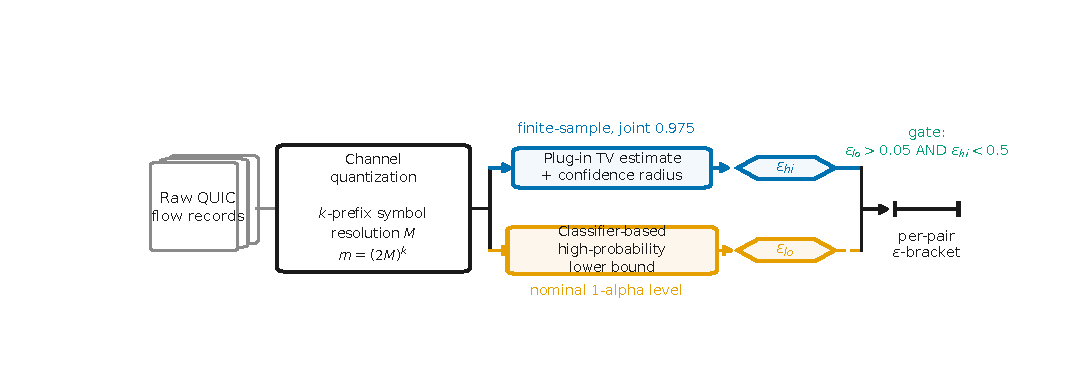
\includegraphics[width=\columnwidth]{figures/paper/fig1_bracket_overview.pdf}
\caption{The EIBO measurement. Raw QUIC flow records are quantized into a
$k$-prefix symbol over a (direction, size) alphabet at resolution $M$. The
quantized symbol feeds two branches that carry different certification
strength: an upper branch combining a plug-in TV estimate with a confidence
radius, which is finite-sample strict, and a lower branch built from a
classifier-based high-probability lower bound, which is asymptotic. The
branches meet at the per-pair interval, whose gate is the conjunction
$\epslo > 0.05$ and $\epshi < 0.5$.}
\label{fig:bracket}
\end{figure}
